\documentclass[11pt]{article}
\usepackage[margin=1in]{geometry}
\usepackage{amsmath,amssymb,amsthm}
\usepackage{booktabs}
\usepackage{algorithm}
\usepackage{algpseudocode}
\usepackage{hyperref}
\usepackage{xurl}
\usepackage{xcolor}
\usepackage{graphicx}
\usepackage[expansion=false]{microtype}
\usepackage{tikz}
\usetikzlibrary{positioning,arrows.meta}
\usepackage{pgfplots}
\pgfplotsset{compat=1.16}

\setlength{\emergencystretch}{3em}
\newtheorem{definition}{Definition}
\newtheorem{lemma}{Lemma}
\newtheorem{theorem}{Theorem}
\newtheorem{remark}{Remark}

\newcommand{\F}{\mathbb{F}_{2^{128}}}
\newcommand{\T}{\mathsf{T}}
\newcommand{\AND}{\textsf{AND}}
\newcommand{\XOR}{\textsf{XOR}}
\newcommand{\blake}{\mathrm{Blake3}}
\newcommand{\todo}[1]{\textcolor{red}{[#1]}}

\title{Garbling a Post-Quantum STARK Verifier for Bitcoin}
\author{GOAT Network Research Group}
\date{}

\begin{document}
\maketitle

\begin{abstract}
BitVM-style protocols verify succinct proofs on Bitcoin by garbling a proof
verifier off-chain. Every garbled verifier and every witness-encryption
alternative proposed so far checks an elliptic-curve SNARK, which a quantum
adversary breaks. A hash-based STARK verifier avoids this but is hard to garble:
it branches on data, its transcript is defined only by an implementation,
hashing dominates its cost, and a stored circuit of $10^8$ gates does not fit in
memory. We garble Plonky3's complete multi-STARK verifier over WHIR, with all
arithmetic in the binary tower field $\F$ and Blake3 for commitments, transcript
and garbling. Additions are free under free-XOR, a multiplication costs
$2{,}187$ \AND{} gates, a Blake3 compression $10{,}281$, and a streaming garbler
holds one byte per wire and a label per live wire. For a Keccak-$f$ trace of
$2^{18}$ rows at 104 bits of soundness, the verifier has 94.1M non-free gates and
garbles to 1.5\,GB in under a minute on one core: about $30\times$ fewer
non-free gates than the Boolean-garbled Groth16 verifier, with no pairing and no
trusted setup. We place it in a BitVM3-style protocol on today's Bitcoin, where a
dispute publishes the proof's million bits: 2.5\,MvB with adaptor signatures,
12 to 17\,MvB with hash-based keys, and a fifth less after tuning the proof. A
quantum analysis shows that the parameters offer about 52 bits against a quantum
adversary, that the 128-bit field caps any configuration near 54, and that 100
quantum bits need 256-bit labels and field, for an estimated $3\times$ the gates.
\end{abstract}

% =====================================================================
\section{Introduction}

Bitcoin cannot verify a succinct proof in Script, but a trust-minimized bridge
needs exactly that. Consider a withdrawal from a rollup: an operator has paid
out a user on Bitcoin and must prove, to a Bitcoin script, that the rollup's
state authorizes the payment; the proof is a STARK over the rollup's execution.
Hashing dominates such statements, and we evaluate on a hash-heavy standard case,
proofs of Keccak-$f$ permutations.

A SNARK verifier written in Script takes hundreds of megabytes~\cite{babe2026}.
The BitVM line of work therefore verifies \emph{optimistically}: a prover claims
a result, and a challenger disputes it only if it is wrong.
BitVM2~\cite{laa25bitvm2} settles a dispute by bisecting the verifier's
execution trace on-chain, which is secure but expensive: a mainnet experiment
put the unhappy path at over \$14{,}000~\cite{babe2026}. BitVM3 moves the
verifier off-chain into a \emph{garbled circuit}~\cite{lin25bitvm3,bitvm3paper,che25sok}.
At setup the verifier circuit is garbled. At dispute time the proof is published
under one-time signatures that give the evaluator the circuit's input labels, and
the outcome depends on which output label the evaluation yields. On-chain, only
the signed proof and a hashlock remain, at tens of dollars~\cite{babe2026}.

The off-chain side is where the existing designs fall short. A garbled circuit
has to be generated, stored for the lifetime of the deposit and checked, because
the garbler may cheat, typically by cut-and-choose over many instances. The
Boolean-garbled Groth16 verifier~\cite{bit25b} has about $3\times10^9$ non-free
gates, some 42\,GiB, and hours of cut-and-choose setup~\cite{babe2026}. Garbling
Groth16 with native group operations~\cite{kflt26native} and witness
encryption~\cite{babe2026} shrink the artifact to megabytes. All of these
designs, however, verify an elliptic-curve SNARK, pairing-based or its
designated-verifier form over BN254 or a binary curve: a quantum adversary breaks
them, and they need a trusted or secret setup. A STARK proof must
first be wrapped in such a SNARK, which reintroduces both.

\paragraph{Key idea.} We garble a hash-based STARK verifier directly and make it
cheap by choosing its field. Under free-XOR~\cite{ks08} a garbled circuit pays
only for non-linear gates, and in a field of characteristic two every addition
is an \XOR. A STARK over the binary tower field $\F$ with Blake3 commitments
therefore costs, as a garbled circuit, little more than its hashes and a
moderate number of field multiplications. Its soundness, commitments, transcript
and garbling PRF all rest on Blake3.

\paragraph{Challenges.} Four problems stand between this idea and a working
garbled verifier.
\begin{itemize}
  \item[C1] \emph{A fixed circuit for a branching verifier.} A garbled circuit has
    one shape for all inputs, while the verifier redraws challenges and fixes
    coordinates depending on sampled values.
  \item[C2] \emph{A transcript defined only by code.} Fiat--Shamir soundness
    requires the circuit to absorb and sample exactly the bytes the prover's
    implementation does, and that byte schedule is not specified outside the
    implementation.
  \item[C3] \emph{Hashing dominates.} Merkle paths, leaf rows and the transcript
    are Blake3 compressions, and a compression costs more than four field
    multiplications.
  \item[C4] \emph{Memory.} A verifier of $10^8$ non-free gates has several
    hundred million wires; a builder that stores the gate list needs tens of
    gigabytes before garbling starts.
\end{itemize}

\paragraph{Contributions.} Each contribution answers one challenge.
\begin{itemize}
  \item \textbf{A fixed-shape circuit for the full verifier (C1, C2).} We
    implement Plonky3's multi-STARK verifier~\cite{plonky3} over the Boolean WHIR
    trace commitment as a Boolean circuit with one output wire: the transcript,
    the zerocheck of the AIR, the batching of the opened columns, the bit ring
    switch and the WHIR opening. Data-dependent branches are fixed and guarded,
    and the transcript follows a byte schedule recovered from Plonky3's own
    verifier, so one circuit serves every proof of a configuration and can be
    garbled before the proof exists (\S\ref{sec:construction}).
  \item \textbf{Cheaper gadgets (C3).} Tower-field multiplication at $3^k$ \AND{}
    gates per $2^k$ bits, with squaring and multiplication by the tower generator
    free, and a Blake3 circuit at $10{,}281$ \AND{} gates per compression instead
    of $20{,}657$, with tree mode for long inputs (\S\ref{sec:gadgets}).
  \item \textbf{A streaming garbler (C4).} A plan pass counts each wire's uses,
    and the garbling pass garbles and checks each gate as the builder emits it and
    releases a wire's slot after its last use (\S\ref{sec:streaming}).
  \item \textbf{A protocol on today's Bitcoin and its cost.} The verifier in a
    BitVM3-style dispute with cut-and-choose, three ways to publish the proof on
    chain, and a sweep of the proof's parameters that bounds how far its
    input shrinks (\S\ref{sec:protocol}).
  \item \textbf{A post-quantum analysis.} Bounds for every component against a
    quantum adversary, from Fiat--Shamir in the quantum random-oracle model to
    Grover search on the garbling offset, and the parameters and cost that
    restore a quantum security target (\S\ref{sec:pq}).
  \item \textbf{Measurements.} Real Keccak-$f$ proofs from $2^5$ to $2^{20}$ rows,
    a gate profile, an ablation of the gadget and memory choices, the on-chain
    cost of a dispute, and a comparison with pairing-based designs
    (\S\ref{sec:eval}).
\end{itemize}
The circuit builder and the measurements are open source; the streaming
garbler, the Blake3 circuit and a label-level evaluator are contributed to
GOAT's bitvm-gc~\cite{bitvmgc}.

% =====================================================================
\section{Setting}\label{sec:setting}

\subsection{Garbled verifiers on Bitcoin}

We follow the BitVM3 setting~\cite{bitvm3paper}. A \emph{garbler}, the operator
who proves, and an \emph{evaluator}, a challenger, agree on a verifier circuit $C$
with one output wire, and $C$ is garbled at setup. At dispute time the operator
publishes its proof on-chain under one-time keys, and each published bit gives
the evaluator the input label of that bit's value. The proof is public, so we use
\emph{privacy-free} garbling: the evaluator may learn every wire's value. What
garbling must provide is \emph{authenticity}. Holding the labels of an input $x$,
the evaluator obtains the label of the output value $C(x)$, and it cannot obtain
the label of the other value. A hashlock on the label of value 0 lets a challenger
who evaluates an invalid proof stop the operator's claim.

The garbler may cheat, so the garbling is checked by cut-and-choose, as in
BABE~\cite{babe2026}, Mosaic~\cite{mosaic26} and bitvm-gc~\cite{bitvmgc}; its cost
is linear in the size of the garbled circuit, which this paper reduces.
Section~\ref{sec:protocol} gives the full protocol and its on-chain cost.

\subsection{The garbling scheme}\label{sec:garbling}

We use privacy-free garbling~\cite{fno15privacyfree} with free-XOR~\cite{ks08}
and one ciphertext per non-free gate, in the syntax of Bellare, Hoang and
Rogaway~\cite{bhr12foundations}.

Let $\Delta$ be a random
secret 128-bit offset. Every wire $w$ has a false label $w_0$, and its true label
is $w_1=w_0\oplus\Delta$. Let $H(\ell,g)=\blake(\ell\,\|\,g)$ truncated to 128
bits, where $g$ is the gate's index. An \XOR{} gate sets $c_0=a_0\oplus b_0$ and
has no ciphertext. An \AND{} gate $c=a\wedge b$ sets
\[
  c_0 = H(a_0,g), \qquad \mathit{ct} = H(a_1,g)\oplus H(a_0,g)\oplus b_0 .
\]
An evaluator holding the label $a$ of value $x$, and $b$ of value $y$, outputs
$H(a,g)$ if $x=0$ and $H(a,g)\oplus\mathit{ct}\oplus b$ if $x=1$. In both cases
this is the label of $x\wedge y$. An \textsf{OR} gate is symmetric, with
$c_0=H(a_1,g)\oplus\Delta$ and $\mathit{ct}=H(a_1,g)\oplus H(a_0,g)\oplus b_1$.
The garbled circuit is one 16-byte ciphertext per \AND{} or \textsf{OR} gate.

Two details matter in practice. First, $\Delta$ must be secret and fresh for
each garbling: with a public $\Delta$ any label yields its complement, and the
output's other label is free to compute. Second, a hash-based PRF gives labels
no algebraic structure. RSA-based garbling proposals for BitVM3 were broken
exactly through such structure: label forgery by extended Euclid on coprime
exponents, and by the Franklin--Reiter related-message
attack~\cite{flb25}.

\subsection{The proof system}

The proof system is Plonky3's multi-STARK~\cite{plonky3} over the Boolean WHIR
trace commitment, with every field in the Wiedemann tower
\[
  \T_0=\mathbb{F}_2,\qquad \T_{k+1}=\T_k[X_k]/(X_k^2+X_{k-1}X_k+1),\qquad X_{-1}=1 ,
\]
up to $\T_7=\F$. An element of $\T_{k+1}$ is stored as its low half (the
coefficient of $1$) and its high half (the coefficient of $X_k$), recursively
down to bits. The trace is committed as bits: a Boolean column is packed into
$\F$ elements, and WHIR commits to the packed multilinear polynomial on an
additive (Cantor) evaluation domain.

\paragraph{Terms.} An \emph{AIR} (algebraic intermediate representation) is a
set of polynomial constraints over a trace's current and next rows. A
\emph{zerocheck} proves that the constraints vanish on every row by a sumcheck
against the equality polynomial $\mathrm{eq}(\tau,\cdot)$ at a random point
$\tau$. \emph{WHIR} is a Reed--Solomon proximity test used as a multilinear
polynomial commitment. Its \emph{STIR queries} open the committed, folded
codeword at random positions, and its \emph{out-of-domain} (OOD) samples bind the
committed polynomial at points outside the evaluation domain. The \emph{Cantor
basis} is the $\mathbb{F}_2$-basis $v_0=1$, $v_i^2+v_i=v_{i-1}$, which gives
binary fields an additive FFT domain. The \emph{bit ring switch} turns a claim
about a polynomial's bits into a claim about its packed $\F$ representation.
\emph{Johnson list-decoding regime} refers to the proximity parameters for which
the soundness bounds are proven via the Johnson bound, without conjectures.

\paragraph{Verification.} The verifier:
\begin{enumerate}
  \item runs a \emph{zerocheck} of the AIR: a degree-4 sumcheck over the row
    variables, then the AIR constraints, evaluated at the bound point from the
    opened current and next rows and Horner-batched under a challenge $\alpha$,
    against $\mathrm{eq}(\tau,r)$;
  \item batches the opened columns into one bit-level claim, at a column point
    drawn from the transcript;
  \item runs the \emph{bit ring switch}, which turns that claim into an $\F$
    claim on the packed polynomial. It uses a $128\times128$ tensor and, above
    $2^7$ rows, its carry and last tensors, a batched sumcheck, and a closing
    weight computed in the tensor algebra;
  \item runs the WHIR opening of that claim: sumcheck rounds with proof of work,
    STIR queries on Merkle-committed folded codewords, and a final polynomial.
\end{enumerate}
All challenges come from a Blake3 sponge over bytes, and all Merkle trees use
Blake3 compressions.

% =====================================================================
\section{The verifier as a circuit}\label{sec:construction}

This section turns the verifier of \S\ref{sec:setting} into a Boolean circuit
with one output wire. Figure~\ref{fig:pipeline} shows its stages in transcript
order, with each stage's share of the non-free gates of our running example: a
$2^{18}$-row Keccak-$f$ trace with 1{,}625 columns, 1{,}650 AIR constraints and
22 packed variables, whose proof is 140\,KiB and whose verifier has 94.1M
non-free gates. We first describe the gadgets, then the transcript, the
multi-STARK layers and WHIR.

\begin{figure}[t]\centering
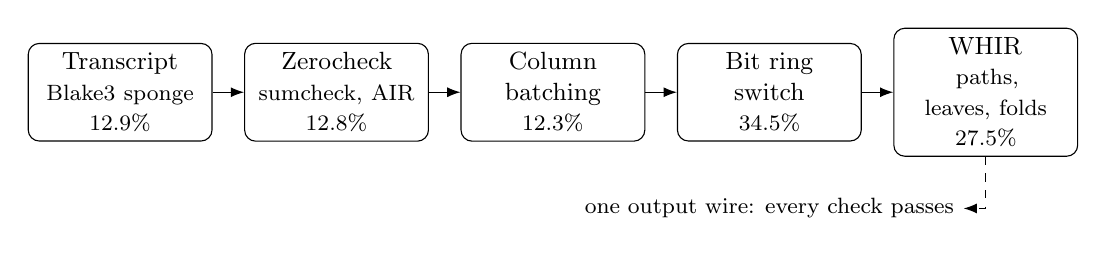
\begin{tikzpicture}[node distance=4mm, box/.style={draw, rounded corners, align=center, font=\small, minimum height=11mm, text width=21mm}]
\node[box] (t) {Transcript\\{\footnotesize Blake3 sponge}\\{\footnotesize 12.9\%}};
\node[box, right=of t] (z) {Zerocheck\\{\footnotesize sumcheck, AIR}\\{\footnotesize 12.8\%}};
\node[box, right=of z] (c) {Column\\batching\\{\footnotesize 12.3\%}};
\node[box, right=of c] (r) {Bit ring\\switch\\{\footnotesize 34.5\%}};
\node[box, right=of r] (w) {WHIR\\{\footnotesize paths, leaves, folds}\\{\footnotesize 27.5\%}};
\draw[-{Latex}] (t) -- (z); \draw[-{Latex}] (z) -- (c); \draw[-{Latex}] (c) -- (r); \draw[-{Latex}] (r) -- (w);
\node[below=6mm of r, font=\footnotesize, align=center] (o) {one output wire: every check passes};
\draw[-{Latex}, dashed] (w.south) |- (o.east);
\end{tikzpicture}
\caption{The ring switch dominates the verifier circuit, followed by WHIR. The
stages appear in transcript order, with each stage's share of the 94.1M non-free
gates of the $2^{18}$-row verifier: transcript is the STARK and WHIR sponges,
zerocheck is its sumcheck, AIR constraints and closing, and WHIR is everything
after the ring switch except its transcript.}
\label{fig:pipeline}
\end{figure}

\subsection{Gadgets}\label{sec:gadgets}

\paragraph{Tower arithmetic.} A wire vector for an element of $\T_k$ is its
bit pattern, so gadget outputs can be read back directly as field elements.
Multiplication follows the tower recursively, Karatsuba at each level:
\[
  z_0=a_0b_0,\quad z_2=a_1b_1,\quad z_1=(a_0+a_1)(b_0+b_1)+z_0+z_2,\qquad
  ab=(z_0+z_2)+(z_1+X_{k-1}z_2)\,X_k .
\]
Additions are free. Multiplication by the generator $X_{k-1}$ is a rewiring plus
\XOR{}s, and squaring is linear over $\mathbb{F}_2$. The only \AND{} gates are
the base-field products, three per level, so a $2^k$-bit multiplication costs
$3^k$ \AND{} gates: $2{,}187$ in $\F$. A multiplication by a constant folds to
\XOR{}s entirely.

\paragraph{Blake3.} We start from bitvm-gc's Blake3 circuit and change two
things. A 32-bit addition's carry is the majority
\[
  \mathrm{maj}(a,b,c)=c\oplus\big((a\oplus c)\wedge(b\oplus c)\big),
\]
one \AND{} per bit, and the carry out of the top bit is discarded, so it is not
computed. This halves a compression from $20{,}657$ to $10{,}281$ \AND{} gates.
We also add Blake3's tree mode (chunk chaining values on a stack, parent nodes,
the root last). The verifier's transcript absorbs more than one 1{,}024-byte
chunk between samples: the final polynomial is 64 coefficients, 1{,}024 bytes
on its own. Table~\ref{tab:gadgets} gives the costs. Every gadget is checked
against the reference implementation (\texttt{p3-binary-field}, the
\texttt{blake3} crate) on random inputs.

\begin{table}[t]\centering\small
\begin{tabular}{lr}\toprule
gadget & \AND{} gates\\\midrule
$\F$ multiplication & 2{,}187\\
$\F$ squaring, multiplication by $X_{k-1}$, addition & 0\\
Blake3 of 64 bytes (a Merkle compression) & 10{,}281\\
Blake3 of 256 bytes (a leaf row of 16 elements) & 41{,}511\\
Blake3 of 1{,}072 bytes (two chunks: a transcript flush) & 186{,}125\\\bottomrule
\end{tabular}
\caption{Gadget costs, checked against \texttt{p3-binary-field} and the
\texttt{blake3} crate.}
\label{tab:gadgets}
\end{table}

\subsection{Transcript}

The transcript is Plonky3's challenger over a Blake3 byte sponge. Observing
appends to an input buffer; sampling, when the output buffer is empty, hashes
the input buffer, replaces it with the digest, and pops bytes from the digest's
end. A field element is 16 little-endian bytes. A query index is 8 bytes read
as a little-endian integer and masked. A proof-of-work check absorbs the
witness and requires a fixed number of sampled bits to be zero. We implement the
same challenger on wires. Its schedule has no data-dependent branch: queries are
a fixed number of masked draws, and a proof-of-work check a fixed number of
bits. So the circuit's shape is a function of the configuration alone. The
sub-transcripts' domain separators are constants, baked in as constant wires,
and everything the prover sends is an input.

The byte schedule, that is, the order in which roots, out-of-domain answers,
sumcheck messages, proof-of-work witnesses, stratified query draws and the final
polynomial are absorbed and sampled, is implicit in Plonky3's implementation and
not specified separately.
We recovered it by running Plonky3's own verifier through a challenger that logs
every byte, and we test the circuit against that log op for op.

\subsection{The multi-STARK layers}

The zerocheck, the column batching and the ring switch are implemented
gate for gate from a reference implementation that is checked op for op against
Plonky3's verifier. The AIR arrives as Plonky3's symbolic constraints and is
evaluated on wires.

Two of Plonky3's data-dependent branches cannot appear in a
fixed circuit. We fix them and guard them with checks.
\begin{itemize}
  \item Plonky3 redraws a zerocheck challenge coordinate that happens to be zero.
    The circuit takes a fixed number of draws and requires each to be nonzero.
  \item Plonky3's ring switch would fix a column-point coordinate that is
    exactly $0$ or $1$. The circuit assumes there is no such coordinate and
    checks it.
\end{itemize}
Each event has probability about $2^{-127}$ per coordinate. When it occurs the
circuit rejects where Plonky3 would continue, never the reverse.

\subsection{WHIR}

The WHIR layer checks every proof-of-work witness. It hashes every opened row and
walks it up its Merkle path to the root absorbed in the transcript. It then folds
each queried row with the round's folding randomness, and checks the final
queries against the final polynomial and the closing sumcheck identity. Plonky3 sends
Merkle openings pruned: siblings that another query can recompute are left out.
A fixed circuit cannot follow a data-dependent frontier, so the proof is expanded
outside the circuit into one full path per query. This costs back the pruning's
savings, and it is the right trade for a circuit whose shape must not depend on
the proof. When the commitment uses a Merkle cap of $2^h$ roots, the transcript
absorbs all of them, and each query selects its root with a multiplexer on the
top $h$ index bits: $256(2^h-1)$ \AND{} gates, against $h$ compressions saved.

% =====================================================================
\section{Streaming garbling}\label{sec:streaming}

The circuits here have $10^8$--$10^9$ non-free gates and several times as many
wires. A builder that stores the gate list, as bitvm-gc's \texttt{CircuitAdapter}
does, needs tens of gigabytes before garbling starts. Upstream's own DV-SNARK
verifier test, for example, exceeds 64\,GB. Nothing in garbling needs the gate
list, though: a gate's ciphertext depends only on its input labels.

Our garbler is a circuit-builder backend that garbles each gate as it is
emitted. It uses two passes of the same deterministic builder
(Algorithm~\ref{alg:stream}). The \emph{plan} pass records, for each wire by
creation index, the number of gates that read it: one byte per wire, with 255
meaning ``never release''. The \emph{garbling} pass hands out slots. A wire's
slot is released after its last read, and a later wire takes it. Wire
identifiers are slots, which the builder interface permits. The two constant
wires, and any wire read after the build (an output), are pinned. Both passes
apply the same constant folding ($x\oplus x=0$, $x\wedge 1=x$, \ldots), so they
see the same wires. Slot storage is chunked, so that a growing array never
reallocates.

\begin{algorithm}[t]
\caption{Streaming garbling of a deterministic builder $\mathcal{B}$}
\label{alg:stream}
\begin{algorithmic}[1]
\State \textbf{plan:} run $\mathcal{B}$ on a backend that only counts: $\mathit{uses}[k]\gets$ reads of the $k$-th created wire
\State pin the constants and the outputs: $\mathit{uses}[k]\gets\infty$
\State \textbf{garble:} $\Delta\gets\{0,1\}^{128}$; run $\mathcal{B}$ again on the backend:
\State \quad on input wire $k$: $\ell_0[s]\gets\blake_{\mathit{seed}}(k)$ in a free slot $s$; $v[s]\gets$ its value
\State \quad on $\XOR(a,b)$: $\ell_0[s]\gets\ell_0[a]\oplus\ell_0[b]$; $v[s]\gets v[a]\oplus v[b]$
\State \quad on $\AND(a,b)$ with gate index $g$:
\State \qquad $(c_0,\mathit{ct})\gets\mathrm{Garble}(\ell_0[a],\ell_0[b],g,\Delta)$; emit $\mathit{ct}$
\State \qquad $e\gets\mathrm{Eval}(\ell_{v[a]}[a],\ell_{v[b]}[b],\mathit{ct},g,v[a])$
\State \qquad $\ell_0[s]\gets c_0$; $v[s]\gets v[a]\wedge v[b]$; \textbf{assert} $e=\ell_{v[s]}[s]$
\State \quad on $\textsf{OR}(a,b)$: as for \AND{}, with the \textsf{OR} garbling of \S\ref{sec:garbling}
\State \quad after each read of $a$: decrement $\mathit{uses}[a]$; release $a$'s slot at zero
\end{algorithmic}
\end{algorithm}

The garbler holds the witness, so it evaluates as it garbles. At each non-free
gate it runs the evaluator's formula on the labels of the actual values, and
requires the result to equal the label of the gate's output value. The circuit
is thereby garbled, evaluated and checked gate by gate on the proof it is built
from. Memory is one byte per wire for the plan, 0.61\,GiB for the 659M wires at
$2^{18}$ rows, plus 18 bytes per live wire (a 16-byte label, the value and a use
counter), 41\,MB at the peak of 2.26M live wires. The plan depends only on the circuit, so every garbled
instance of a configuration can share it. The same code
garbles bitvm-gc's DV-SNARK verifier in 2.2\,GB (\S\ref{sec:eval}).

% =====================================================================
\section{Security}\label{sec:security}

This section states what the garbled verifier guarantees and on which
assumptions. It combines the soundness of the proof system, the effect of the two
guarded branches, and the authenticity of the garbling.

\paragraph{The circuit and the verifier.} When neither guarded event of
\S\ref{sec:construction} occurs, the circuit computes exactly Plonky3's verifier;
we test this op for op against Plonky3's logged transcript and on real proofs.
When a guarded event occurs, the circuit outputs 0. Hence an output of 1 implies
that Plonky3's verifier accepts, and an honest proof is rejected only if a guarded
event occurs, with probability at most $\varepsilon_{\mathrm{guard}}\approx
n\cdot2^{-127}$ for $n$ guarded coordinates.

\paragraph{Soundness of the proof system.} We use Plonky3's own security
assessment of each configuration. Every term is a proven bound, the proximity
terms in the Johnson list-decoding regime, and nothing is left unassessed
(Table~\ref{tab:security}).
At $2^{18}$ rows the binding term is the WHIR opening at $104.3$ bits (110 bits per
term, rate $1/32$, folding factor 4, proof of work up to 32 bits). The other terms
are constraint batching $109.0$, zerocheck $114.5$ and its sumcheck $113.5$, bit
ring switch $114.0$, column batching $115.2$, and commitment and transcript
collisions $128$ (Blake3). We write $\varepsilon_{\mathrm{STARK}}(t)$ for the
composed error against an adversary making $t$ hash queries. Plonky3's report
states it as bits of security, $104.3$ at $2^{18}$ rows, meaning that
$\varepsilon_{\mathrm{STARK}}(t)\le t\cdot2^{-104.3}$ for a classical adversary; \S\ref{sec:pq} gives the quantum bound.

\begin{table}[t]\centering\small
\begin{tabular}{lrrrrrr}\toprule
trace rows & $2^5$ & $2^8$ & $2^{12}$ & $2^{16}$ & $2^{18}$ & $2^{20}$\\\midrule
composed soundness (bits) & 106.1 & 105.2 & 104.7 & 104.3 & 104.3 & 104.0\\\bottomrule
\end{tabular}
\caption{Soundness stays at about 104 bits at every measured size, 103.95 at $2^{20}$ rows. The values are
Plonky3's composed soundness for each configuration.}
\label{tab:security}
\end{table}

\paragraph{Authenticity of the garbling.} Our scheme is privacy-free
garbling~\cite{fno15privacyfree} with free-XOR~\cite{ks08} and one ciphertext per
non-free gate~\cite{zre15}, with $H=\blake$ and a fresh secret $\Delta$ per
garbling. Free-XOR is secure when $H$ is circular correlation
robust~\cite{ckkz12freexor}; we assume this of Blake3, as is standard for
hash-based garbling. In the BitVM setting the garbled circuit is published at
setup and the proof is chosen afterwards, so authenticity must hold for inputs
chosen adaptively, after the garbled circuit is seen~\cite{bhr12adaptive}. Let
$\varepsilon_{\mathrm{GC}}$ be the advantage of an evaluator that sees the garbled
circuit, then chooses an input $x$, receives its labels, and outputs the label of
the value $\neg C(x)$ on the output wire. We assume that our Blake3-based
free-XOR garbling has adaptive authenticity in this sense, with Blake3 modelled as
a random oracle; Bellare, Hoang and Rogaway give constructions proven adaptively
secure~\cite{bhr12adaptive}.

\begin{theorem}\label{thm:main}
Let $C$ be a correctly garbled verifier of a fixed configuration, and $x$ the
encoding of a proof $\pi$ for a statement.
\begin{enumerate}
  \item[(i)] \emph{Soundness.} If the statement is false, an evaluator holding the
    labels of $x$ obtains the output label of value 0, except with probability at
    most $\varepsilon_{\mathrm{STARK}}(t)$, where $t$ bounds the hash queries of
    the party that chose $\pi$.
  \item[(ii)] \emph{Authenticity.} If $\pi$ is honestly generated, an evaluator
    holding the labels of $x$ obtains the output label of value 0 with probability
    at most $\varepsilon_{\mathrm{guard}}+\varepsilon_{\mathrm{GC}}$.
\end{enumerate}
\end{theorem}

\noindent\emph{Proof sketch.} (i) If $C(x)=1$, Plonky3's verifier accepts $\pi$ by
the previous paragraphs, which for a false statement happens with probability at
most $\varepsilon_{\mathrm{STARK}}(t)$. Otherwise $C(x)=0$, and correctness of the
garbling yields the label of value 0. (ii) For an honest proof $C(x)=1$ unless a
guarded event occurs, and the label of value 0 is then the label of $\neg C(x)$,
which the evaluator obtains with probability at most
$\varepsilon_{\mathrm{GC}}$. \hfill$\square$

\smallskip\noindent Section~\ref{sec:protocol} uses (i) to protect challengers
against a false claim and (ii) to protect an honest operator.

\subsection{Post-quantum analysis}\label{sec:pq}

No step of the construction uses a number-theoretic assumption: the proof
system, the commitments, the transcript and the garbling rely on Blake3 alone.
Pairing-based verifiers (Groth16, Pari and their designated-verifier variants),
the witness-encryption schemes built on them (\S\ref{sec:related}) and Bitcoin's
own Schnorr signatures fall to Shor's algorithm~\cite{shor94}. Our verifier does
not. Relying on hashing alone is necessary for post-quantum security but not
sufficient~\cite{zkmhashpq}: a quantum adversary still speeds up generic search
over hash inputs. This subsection bounds that speed-up for every component and
gives parameters that restore a target level. Table~\ref{tab:pq} summarises it.

\paragraph{Fiat--Shamir against quantum adversaries.} In the quantum random-oracle
model, Chiesa, Manohar and
Spooner~\cite{cms19qrom} show that compiling a public-coin interactive oracle
proof with round-by-round soundness error $\varepsilon_{\mathrm{rbr}}$ with a hash
bounds the success of a quantum adversary that makes $t$ hash queries by
$O(t^2\varepsilon_{\mathrm{rbr}}+t^3/2^{\lambda})$, where $\lambda=256$ is the
digest length. A classical adversary is bounded by
$O(t\,\varepsilon_{\mathrm{rbr}})$.

WHIR has round-by-round soundness~\cite[\S5]{whir25}. For the
sumcheck-based layers (zerocheck, column batching, ring switch) we assume it, as
is standard for sumcheck, with each of Plonky3's terms as the round error. A
round with error $2^{-a}$ therefore offers about $a/2$ bits
against a quantum adversary, and Grover search~\cite{grover96} attains this
generically when the bad challenges form an unstructured set. Proof-of-work
grinding is generic search too: $b$ bits of grinding cost $2^{b}$ hashes
classically and about $2^{b/2}$ quantumly.

\paragraph{The proof system at our parameters.} At $2^{18}$ rows each WHIR term
targets 110 bits, of which grinding supplies 26 to 32 bits (per round: 33
queries with 30 and 28 bits of grinding, 20 with 32 and 30, 15 with 29 and 32, and
12 terminal queries with 27). Both parts halve under quantum search, so each WHIR
term offers about 55 bits, and the composed $104.3$ bits become about 52. The
algebraic terms (zerocheck $114.5$, its sumcheck $113.5$, ring switch $114.0$,
column batching $115.2$, constraint batching $109.0$) are Schwartz--Zippel errors
over the $2^{128}$-element field and offer 54 to 58 bits. They are capped by the
field: no number of queries raises them. Collisions in the 256-bit Blake3
digests cost about $2^{85}$ quantum queries~\cite{bht98}, and preimages
$2^{128}$.

\paragraph{The ceiling of the current configuration space.} Raising Plonky3's
per-term target does not raise the quantum level. We searched the target that
the proven-list-decoding profile accepts at $2^{18}$ rows. Up to 134 bits per term
it keeps the queries at $33+20+15+12$ and raises the grinding to 51--56 bits,
its ceiling; at 200 bits it refuses, needing 103 bits of grinding. Plonky3's
security report fully assesses targets up to 117 bits per term, where the
composed soundness is $108.6$ bits, bound by constraint batching at $109.0$, a
field-size term no WHIR parameter moves. Grinding and the field-bound terms both
halve under quantum search, so no configuration of the current proof system
exceeds about 54 quantum bits. Reaching a quantum target is a change to the
proof system, not to its parameters.

\paragraph{The garbling.} Authenticity rests on the secrecy of $\Delta$, and
$\Delta$ can be tested against a single gate. An evaluator holding the labels
$a,b$ of an \AND{} gate with known values $x,y$ and its ciphertext $\mathit{ct}$
checks a candidate $\Delta'$ by recomputing $\mathit{ct}$ from
$a,a\oplus\Delta',b$ and $\Delta'$. A wrong candidate passes with probability
$2^{-128}$. Grover search therefore recovers $\Delta$ with about $2^{64}$
quantum evaluations of Blake3, after which every label's complement is known
and the output label of the other value is free. With 128-bit labels the
garbling offers about 64 bits against a quantum adversary. The same holds for a
hashlock on a 128-bit output label: a preimage search over $2^{128}$ labels costs
about $2^{64}$. Grover search is highly sequential, and the adversary has only the
time between setup and the end of the dispute window, but we do not rely on
this.

\paragraph{The surrounding protocol.} The protocol of \S\ref{sec:protocol}
publishes input bits under one-time keys. Lamport and Antichain Winternitz keys
rest on \texttt{HASH160} preimages, which cost about $2^{80}$ quantum queries.
Schnorr adaptor signatures, the committee's pre-signed transactions and any
Taproot key path fall to Shor's algorithm. A post-quantum deployment therefore
needs hash-based input keys, which the protocol supports at $5$ to $7\times$ the
on-chain cost of adaptor signatures (Table~\ref{tab:onchain}), and post-quantum
signatures in Bitcoin itself for the pre-signed graph, which no current opcode
provides.

\begin{table}[t]\centering\small
\resizebox{\textwidth}{!}{\begin{tabular}{llrrl}\toprule
component & attack & classical & quantum, as measured & to reach $\lambda_Q$ quantum bits\\\midrule
WHIR opening & FS search, grinding & 104.3 (max.\ 111.3) & $\approx52$ & $\approx2\lambda_Q$ per term: $\approx2.1\times$ queries at $\lambda_Q=100$\\
zerocheck, sumchecks, ring switch & FS search & 109--115 & $\approx54$--$58$ & a field of $\gtrsim2^{2\lambda_Q+14}$ elements: $\mathbb{F}_{2^{256}}$\\
Merkle and transcript hash & collision, preimage & 128 & $\approx85$ & unchanged (256-bit Blake3)\\
garbling ($\Delta$, output hashlock) & Grover on 128-bit labels & 128 & $\approx64$ & $2\lambda_Q$-bit labels: 256 bits\\
hash-based input keys & preimage of \texttt{HASH160} & 160 & $\approx80$ & a 256-bit hash for $\lambda_Q>80$\\
adaptor keys, pre-signed graph & Shor & -- & broken & hash-based keys; post-quantum signatures in Bitcoin\\\bottomrule
\end{tabular}}
\caption{Against a quantum adversary the current parameters offer about 52 bits,
half their classical level; restoring 100 bits needs more queries, a 256-bit field,
256-bit labels and a 256-bit input hash, and signatures that Bitcoin does not
yet offer. Bits of security per component, classically and against a
quantum adversary under the generic square-root speed-up.}
\label{tab:pq}
\end{table}

\paragraph{Parameters for a quantum target.} To offer $\lambda_Q$ bits against a
quantum adversary, every classical term must reach about $2\lambda_Q$ bits.
Three changes follow.
\begin{itemize}
  \item The WHIR terms need about $2\lambda_Q$ bits each. Since grinding also
    halves, the query count must carry most of it: from about 80
    information-theoretic bits per term today to about 168 at $\lambda_Q=100$,
    about $2.1\times$ the queries. Plonky3's profile raises grinding instead,
    so this needs a query-heavy profile.
  \item The algebraic terms need challenges from a field of about
    $2^{2\lambda_Q+14}$ elements, which means one more tower level,
    $\mathbb{F}_{2^{256}}$, at $3^8=6{,}561$ \AND{} gates per multiplication, three
    times today's. Repeating each algebraic check with independent challenges is
    an alternative at a similar cost.
  \item Labels of $2\lambda_Q$ bits: 256-bit labels double the ciphertext size to
    32 bytes per non-free gate. The gate count is unchanged, because labels feed
    the garbling hash, not the circuit.
\end{itemize}
Applying these factors to the measured $2^{18}$ profile gives an estimate, not a
measurement. Merkle paths and leaf hashes scale with the query count ($2.1\times$),
and leaves also with the element size ($2\times$), to about 45M gates. The
transcripts absorb twice the bytes, about 24M. Multiplications triple, and those
that depend on the queries also scale with them, to about 213M. That is about
280M non-free gates, $3\times$ today's, and about 9\,GB garbled at 32 bytes per
gate: about $10\times$ fewer non-free gates than the Boolean-garbled Groth16
verifier, which offers no quantum security at all.

% =====================================================================
\section{Verifying on Bitcoin}\label{sec:protocol}

This section places the garbled verifier in a protocol that today's Bitcoin
enforces, without a soft fork or a data-availability assumption, and prices it.
We take BitVM3's roles~\cite{bitvm3paper,mosaic26}: the operator, who is the
prover, garbles, and challengers evaluate. The running application is a bridge:
the operator has paid a withdrawal from its own funds and claims reimbursement
from a deposit, backed by a stake that it loses if a challenger shows the claim
false.

\paragraph{Setup.} The operator garbles $N$ instances of $C$ from independent
seeds. A challenger chooses $N-M$ of them to open, re-garbles each opened
instance from its seed and compares. The streaming garbler does this in one
garbling pass per instance, reusing the plan that all instances share
(\S\ref{sec:streaming}). The challenger stores the $M$ kept instances, 1.5\,GB
each at $2^{18}$ rows. For each kept instance $j$ the operator commits
$h_j=\mathrm{SHA256}(\ell^j_0)$, the hash of the label of output value 0
(reject). It also fixes
one-time keys for the input bits of $C$, and the kept instances' input labels
are \emph{soldered} to them: publishing bit $b$ of input $i$ under the keys gives
a challenger the label of value $b$ on wire $i$ in every kept instance, and no
other label. The transactions below are pre-signed at setup by a committee, as in
BitVM2~\cite{laa25bitvm2}; as there, their enforcement needs one honest signer.

\begin{figure}[t]\centering
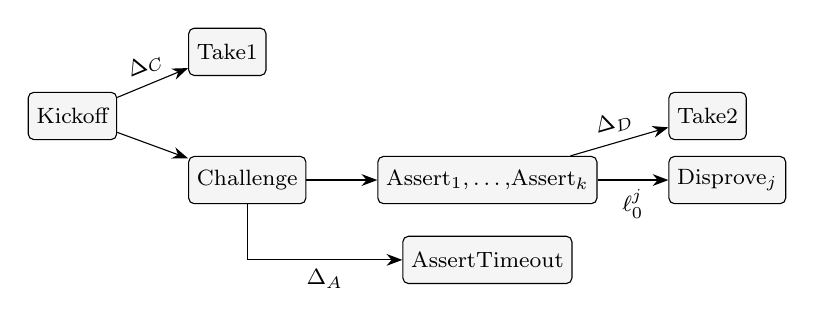
\begin{tikzpicture}[node distance=5mm and 9mm, font=\footnotesize,
  tx/.style={draw, rounded corners=2pt, minimum height=6mm, inner sep=3pt, fill=gray!8},
  arr/.style={-{Stealth[length=2mm]}}]
\node[tx] (kick) {Kickoff};
\node[tx, above right=2mm and 9mm of kick] (take1) {Take1};
\node[tx, below right=2mm and 9mm of kick] (chal) {Challenge};
\node[tx, right=of chal] (assert) {Assert$_1,\dots,$Assert$_k$};
\node[tx, above right=2mm and 9mm of assert] (take2) {Take2};
\node[tx, right=of assert] (disprove) {Disprove$_j$};
\node[tx, below=4mm of assert] (noassert) {AssertTimeout};
\draw[arr] (kick) -- node[above, sloped] {$\Delta_C$} (take1);
\draw[arr] (kick) -- (chal);
\draw[arr] (chal) -- (assert);
\draw[arr] (chal) |- node[pos=0.75, below] {$\Delta_A$} (noassert);
\draw[arr] (assert) -- node[above, sloped] {$\Delta_D$} (take2);
\draw[arr] (assert) -- node[below] {$\ell^j_0$} (disprove);
\end{tikzpicture}
\caption{The dispute costs one challenge and the operator's reveal of the proof;
the happy path costs two constant-size transactions. Pre-signed transactions of one
claim. Labels on edges are relative timelocks, and Disprove$_j$ spends a hashlock
on $h_j=\mathrm{SHA256}(\ell^j_0)$, one leaf per kept instance $j$. Take1 and Take2 pay the operator;
Disprove and AssertTimeout burn its stake, with a reward to the challenger.}
\label{fig:graph}
\end{figure}

\paragraph{Transactions.} Figure~\ref{fig:graph} shows the graph of one claim.
\begin{itemize}
  \item \emph{Kickoff}: the operator claims reimbursement for a withdrawal it has
    paid. If no challenge follows within $\Delta_C$, \emph{Take1} pays it. This is
    the happy path.
  \item \emph{Challenge}: any challenger may spend Kickoff's challenge output,
    paying the operator a bond that covers the cost of Assert, as BitVM2's
    crowdfunded challenge does~\cite{laa25bitvm2}.
  \item \emph{Assert$_1,\dots,$Assert$_k$}: the operator publishes the bits of its
    proof under the one-time keys. The proof is a million bits
    (Table~\ref{tab:main}), so Assert is split into $k$ standard transactions. If
    Assert is not complete within $\Delta_A$, \emph{AssertTimeout} burns the stake.
  \item \emph{Disprove$_j$}: within $\Delta_D$ of the last Assert, a challenger that
    holds $\ell^j_0$ for some kept instance $j$ spends the Assert output through the
    leaf $\texttt{OP\_SHA256}\ h_j\ \texttt{OP\_EQUAL}$, which burns the stake and
    makes \emph{Take2} unspendable. Otherwise Take2 pays the operator after
    $\Delta_D$.
\end{itemize}
The statement's public inputs, such as the rollup state that authorizes the
withdrawal, are committed in Kickoff under the same kind of keys and are input
bits of $C$; the Keccak-$f$ AIR we measure has none.

\paragraph{Dispute.} A challenger reads the published bits from the chain,
obtains through the soldering the input labels of every kept instance, and
evaluates each instance. The evaluation takes one Blake3 call per non-free gate,
half of what garbling takes, and runs off-chain. If the proof is invalid, a correctly garbled
instance yields $\ell^j_0$, and the challenger publishes Disprove$_j$, a hashlock
spend of constant size. Nothing on-chain depends on the size of $C$; only Assert
depends on the size of the proof.

\paragraph{Security.} Let $\varepsilon_{\mathrm{cc}}$ bound the probability
that every kept instance is malformed while every opened one is correct; for
choosing $N-M$ of $N$ uniformly this is $1/\binom{N}{M}$, which is $2^{-40}$ at
$(N,M)=(181,7)$~\cite{babe2026}. Let $\varepsilon_{\mathrm{sol}}$ bound a failure of
the soldering, and $\varepsilon_{\mathrm{sig}}$ a forgery of the one-time keys.
Theorem~\ref{thm:main} then gives two properties, assuming the
committee's graph is enforced and transactions confirm within their timelocks.
\begin{itemize}
  \item \emph{A false claim is disproved.} If the operator's statement is false, an
    honest challenger obtains some $\ell^j_0$ except with probability
    $\varepsilon_{\mathrm{STARK}}(t)+\varepsilon_{\mathrm{cc}}+\varepsilon_{\mathrm{sol}}$:
    a correctly garbled kept instance exists, its labels are those of the published
    proof, and Theorem~\ref{thm:main}(i) applies. An operator that publishes no
    proof loses its stake to AssertTimeout.
  \item \emph{An honest operator keeps its stake.} If the operator's proof is
    honest, no challenger obtains any $\ell^j_0$ except with probability
    $M(\varepsilon_{\mathrm{guard}}+\varepsilon_{\mathrm{GC}})+\varepsilon_{\mathrm{sol}}+\varepsilon_{\mathrm{sig}}$,
    by Theorem~\ref{thm:main}(ii) and a union bound over the kept instances.
\end{itemize}
This is a sketch, not a proof in a ledger model; BitVM3~\cite{bitvm3paper} and
BABE~\cite{babe2026} give such proofs for their instantiations, whose structure
ours follows.

\paragraph{Publishing the input.} Three one-time schemes can carry the input
bits, and they trade on-chain size against assumptions.
\begin{itemize}
  \item \emph{Lamport.} Each bit has two hashed 16-byte preimages. The leaf script
    per bit,
    \begin{center}\ttfamily\small OP\_HASH160 OP\_DUP $h_0$ OP\_EQUAL OP\_SWAP $h_1$ OP\_EQUAL OP\_BOOLOR OP\_VERIFY\end{center}
    is 49 bytes, and the witness 17 bytes. We executed it with 998 bits per
    input, the most that the 1{,}000-item stack limit allows, and it rejected wrong
    preimages. With per-input overhead this is 66.2 weight units, or $16.55$\,vB,
    per bit.
  \item \emph{Antichain Winternitz.} Plain Winternitz chains are unsafe here: from
    a published chain value the evaluator hashes forward to the labels of other
    digit values~\cite{antichain26}. Antichain Winternitz closes this and costs
    $11.31$\,vB per bit at parameters $(2,16)$, with $0.256$\,kB of off-chain table
    per bit; its larger parameters save more on-chain but need up to
    $43.8$\,kB per bit off-chain~\cite{antichain26}, 46\,GB for our input.
  \item \emph{Schnorr adaptor signatures} over 8-bit digits, as in BitVM3 and
    Mosaic: 9{,}707 weight units for a 1{,}024-bit proof~\cite{bitvm3paper}, or
    $2.37$\,vB per bit. Mosaic solders all kept instances to one set of
    signatures by polynomial label correlation, with an on-chain footprint
    independent of the number of instances~\cite{mosaic26}. The signatures rest on
    discrete logarithms, and an evaluator that holds the signing key can spend
    without completing the adaptor~\cite{antichain26}.
\end{itemize}
Our labels are free-XOR correlated, so a hash-based preimage $s$ cannot itself be
a label. It is mapped to one by a translation ciphertext
$\mathrm{KDF}(s)\oplus w_b$, two per input bit and instance: 32 bytes per bit,
33\,MB per instance at $2^{18}$ rows, off-chain. Soldering hash-based keys to $M$
kept instances without publishing $M$ sets needs a proof that the opened and kept
translations agree, as BABE's zero-knowledge soldering~\cite{babe2026} or Glock's
verifiable secret sharing~\cite{eag25glock} provide for smaller inputs. We have not
built it for a million input bits, and its cost there is open.

% =====================================================================
\section{Evaluation}\label{sec:eval}

The experiments answer five questions: how the garbled verifier scales with the
trace (Table~\ref{tab:main}, Figure~\ref{fig:scaling}), where its gates go
(Table~\ref{tab:profile}), how much each design choice contributes (the
ablation), what a dispute costs on-chain and how far its input shrinks
(Tables~\ref{tab:onchain} and~\ref{tab:inputs}), and how it compares with
pairing-based designs (Table~\ref{tab:compare}).

\paragraph{Setup.} We proved Keccak-$f$ permutations with Plonky3's
1{,}625-column characteristic-2 Keccak AIR (booleanity is not constrained,
since the commitment is to bits). A byte-logging challenger recorded each run,
our reference replayed Plonky3's verifier byte for byte, and the full circuit was
then streamed through the garbler. The parameters were rate $1/32$, folding
factor 4 and 110 bits per WHIR term. Garbling was single-threaded. Every run up to
$2^{18}$ rows was limited to 32\,GB of RAM and 8 cores of an Intel Xeon Platinum
8375C at 2.9\,GHz; the $2^{20}$ run, whose proof took longer to generate, ran on
an AMD EPYC 9355 limited to 128\,GB and 32 cores.

The circuit's size depends on the AIR: the transcript, the column combination
and the constraint evaluation grow with the number of columns and constraints.
All sizes below are therefore for this 1{,}625-column AIR, which is a demanding
case; a Groth16 verifier, by contrast, has the same size for every statement.

\paragraph{Scaling.} Table~\ref{tab:main} and Figure~\ref{fig:scaling} give the
full verifier from $2^5$ to $2^{20}$ rows. Every circuit accepted its proof, and
at $2^5$ and $2^8$ we also checked that it rejected the proof with one opened
value changed. Growing the trace $32{,}768$-fold grew the circuit $2.2$-fold,
because the verifier depends on the trace length only through the logarithmic
number of variables.

\paragraph{Garbling efficiency.} To compare garbled verifiers across trace sizes
and AIRs, we define the \emph{garbling efficiency} of a configuration as
\[
  \eta \;=\; \frac{|\mathsf{GC}|}{R\cdot W}\quad\text{bytes per committed cell},
\]
where $|\mathsf{GC}|$ is the garbled circuit's size in bytes, 16 per non-free
gate, $R$ the number of trace rows and $W$ the number of committed columns. It is a
cost per unit of verified computation, so smaller is better. For our Keccak-$f$
AIR, $W=1{,}625$ and each cell is one bit. Because $|\mathsf{GC}|$ grows with
$\log R$ while $R\cdot W$ grows with $R$, $\eta$ falls almost in inverse
proportion to the trace: from $13{,}715$ bytes per cell at $2^5$ rows to $3.53$ at
$2^{18}$ and $0.94$ at $2^{20}$ (Table~\ref{tab:main}). At $2^{20}$ rows the garbled
verifier is smaller than the trace it verifies, 7.5 garbled bits per committed
bit, or 38\,kB per Keccak-$f$ permutation. A verifier of fixed size, such as a
Groth16 verifier, has $\eta$ inversely proportional to the computation its proof
covers as well; comparing $\eta$ across proof systems therefore needs the same
computation and cells of the same kind, bits here against field elements in a
prime-field AIR.

\begin{figure}[t]\centering
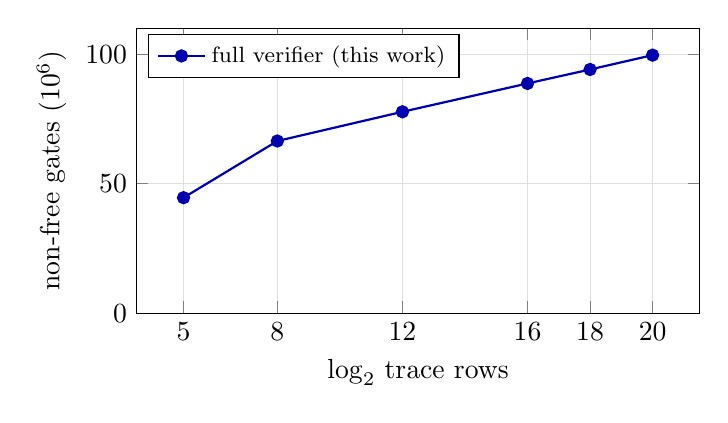
\begin{tikzpicture}
\begin{axis}[width=0.72\textwidth, height=5.2cm, xlabel={$\log_2$ trace rows}, ylabel={non-free gates ($10^6$)},
  xtick={5,8,12,16,18,20}, ymin=0, ymax=110, grid=major, grid style={gray!25}, mark size=2pt,
  legend style={font=\footnotesize, at={(0.02,0.98)}, anchor=north west}]
\addplot[thick, mark=*, color=blue!70!black] coordinates {(5,44.573) (8,66.460) (12,77.736) (16,88.681) (18,94.070) (20,99.614)};
\addlegendentry{full verifier (this work)}
\end{axis}
\end{tikzpicture}
\caption{The garbled verifier grows logarithmically with the trace: from 44.6M
non-free gates at $2^5$ rows to 99.6M at $2^{20}$, $2.2\times$ for a
$32{,}768\times$ larger trace. The Boolean-garbled Groth16 verifier, at about
3{,}000M non-free gates, is off the scale.}
\label{fig:scaling}
\end{figure}

\begin{table}[t]\centering\small
\resizebox{\textwidth}{!}{\begin{tabular}{lrrrrrrr}\toprule
trace & vars & non-free gates & garbled & $\eta$ (B/cell) & garbling & garbler memory & input bits\\\midrule
$2^5$ rows (1 Keccak-$f$) & 9 & 44{,}573{,}121 & 713\,MB & 13{,}715 & 35\,s & 0.32\,GiB & 586{,}240\\
$2^8$ rows (10) & 12 & 66{,}459{,}859 & 1{,}063\,MB & 2{,}556 & 53\,s & 0.46\,GiB & 743{,}808\\
$2^{12}$ rows (163) & 16 & 77{,}736{,}394 & 1{,}243\,MB & 186.9 & 53\,s & 0.54\,GiB & 874{,}240\\
$2^{16}$ rows (2{,}621) & 20 & 88{,}680{,}747 & 1{,}418\,MB & 13.32 & 66\,s & 0.61\,GiB & 997{,}760\\
$2^{18}$ rows (10{,}485) & 22 & \textbf{94{,}069{,}548} & \textbf{1{,}505\,MB} & \textbf{3.53} & 57\,s & 0.65\,GiB & 1{,}041{,}024\\
$2^{20}$ rows (41{,}943) & 24 & 99{,}613{,}898 & 1{,}593\,MB & 0.94 & 42\,s$^{\dagger}$ & 0.68\,GiB & 1{,}108{,}992\\\bottomrule
\end{tabular}}
\caption{The full verifier stays below 100M non-free gates and 1.6\,GB garbled up
to $2^{20}$ rows, and the garbler needs less than 0.7\,GiB. Measured on real
Keccak-$f$ proofs; ``vars'' is the number of packed variables WHIR opens,
garbled size is 16 bytes per non-free gate, and $\eta$ is the garbled size per
committed trace cell, $1{,}625$ columns times the rows. Garbling is single-threaded, and its
time varied by up to 50\% with load on the shared machine (23--35\,s at $2^5$
across runs). Garbler memory is the plan (one byte per wire) plus 18 bytes per
live wire at the peak, computed from the measured counts; at $2^{18}$ rows the
garbler holds at most 2{,}256{,}536 labels live. $^{\dagger}$The $2^{20}$ proof was
generated on a second, larger machine, where the circuit was also garbled, again
on one core.}
\label{tab:main}
\end{table}

\paragraph{Where the gates go.} Table~\ref{tab:profile} breaks the $2^{18}$
circuit down by the verifier phase that emits each gate. The multi-STARK layers
account for $70.8\%$ and WHIR for $29.2\%$. Three of the largest items, the STARK
transcript, the column combination and the AIR constraints, grow with the number
of columns, so a narrower AIR shrinks them directly. The largest single
item is the ring switch closing: 256 multiplications per packed variable, plus a
fixed $11\times512$ for the column selector.

\begin{table}[t]\centering\small
\begin{tabular}{lrr}\toprule
phase & non-free gates & share\\\midrule
ring switch closing & 31{,}633{,}960 & 33.6\%\\
WHIR Merkle paths & 14{,}613{,}722 & 15.5\%\\
column combination & 11{,}582{,}352 & 12.3\%\\
AIR constraints (1{,}650, Horner under $\alpha$) & 10{,}736{,}110 & 11.4\%\\
STARK transcript & 10{,}531{,}194 & 11.2\%\\
WHIR leaf hashes & 3{,}320{,}880 & 3.5\%\\
WHIR closing query weights & 3{,}069{,}960 & 3.3\%\\
WHIR query folds & 2{,}624{,}400 & 2.8\%\\
WHIR transcript & 1{,}603{,}940 & 1.7\%\\
zerocheck sumcheck & 1{,}227{,}336 & 1.3\%\\
ring switch statement & 835{,}688 & 0.9\%\\
other (9 phases) & 2{,}290{,}006 & 2.4\%\\\midrule
total & 94{,}069{,}548 & 100\%\\\bottomrule
\end{tabular}
\caption{A third of the $2^{18}$-row verifier is the ring switch closing, and the
five largest phases make up 84\%. Non-free gates by the verifier phase that emits
them.}
\label{tab:profile}
\end{table}

\paragraph{WHIR alone, and its parameters.} Garbling only the WHIR opening of a
$2^{18}$-variable polynomial (rate $1/32$, folding 4, $35+22+16$ queries) cost
$24.3$M non-free gates with single-root commitments, and $21.2$M with a Merkle
cap of 32 roots. That cap is Plonky3's recommended height and was the optimum in
our sweep of 1 to 256 roots. Three quarters of the WHIR circuit was hashing.
Across rates $1/16$--$1/64$ and folding factors 2--5, rate $1/32$ with folding 4
gave the smallest circuit among the configurations we kept; rate $1/64$ saved a
further $10\%$ of gates at the price of a prover domain twice as large.

\paragraph{Why a binary field.} We also built KoalaBear
($p=2^{31}-2^{24}+1$) and Poseidon2 on wires, to price the prime-field
alternative. A KoalaBear multiplication is $3{,}451$ \AND{} gates, and a
degree-4 extension multiplication $60{,}615$, against $2{,}187$ for all of
$\F$. One Poseidon2 permutation of width 16 is $1{,}240{,}747$ \AND{} gates:
$120$ Blake3 compressions. The WHIR opening of a $2^{20}$ KoalaBear
configuration (2{,}157 permutations, about 7{,}500 extension multiplications)
would be about $3.1\times10^9$ gates with Poseidon2, more than the whole
Boolean-garbled Groth16 verifier, and still $0.3$--$0.5\times10^9$ with Blake3,
against our $21$M for a $2^{18}$-variable opening. The four-fold difference in
size does not account for a gap of $15$ to $150\times$: a garbled STARK verifier
should use a binary field.

\paragraph{Ablation.} Table~\ref{tab:ablation} isolates two of our choices on
the full verifier. Replacing our Blake3 adder with the original two-\AND{} adder,
with everything else unchanged, grew the circuit by $32\%$ at $2^5$ rows and
$29\%$ at $2^8$: the adder saves a quarter of the whole verifier, because Blake3
is in the transcript, the leaf hashes and every Merkle path. Building the same
$2^5$-row verifier as a stored circuit produced exactly the same gates and wires,
but took 12.4\,GiB and 283\,s, against 0.69\,GiB and 33\,s for the plan and the
streamed garbling together, including the garbling itself.

\begin{table}[t]\centering\small
\begin{tabular}{lrrr}\toprule
configuration & non-free gates & peak memory & time\\\midrule
$2^5$ rows, this work (streamed) & 44{,}573{,}121 & 0.69\,GiB & 33\,s (plan + garble)\\
$2^5$ rows, stored build & 44{,}573{,}121 & 12.4\,GiB & 283\,s (build only)\\
$2^5$ rows, original Blake3 adder & 58{,}997{,}590 ($+32\%$) & -- & --\\\midrule
$2^8$ rows, this work & 66{,}459{,}859 & -- & --\\
$2^8$ rows, original Blake3 adder & 85{,}768{,}603 ($+29\%$) & -- & --\\\bottomrule
\end{tabular}
\caption{The one-\AND{} adder removes about a quarter of the verifier's gates, and
streaming cuts memory $18\times$. Peak memory is the whole process's, including
proof generation, which is negligible at $2^5$ rows; the stored build's time
excludes garbling.}
\label{tab:ablation}
\end{table}

\paragraph{On-chain cost.} Table~\ref{tab:onchain} prices a dispute at $2^{18}$
rows. The happy path, Kickoff and Take1, and the Challenge and Disprove
transactions have constant size; BitVM3 reports its Disprove at 93\,vB, and ours
is the same hashlock spend~\cite{bitvm3paper}. Assert carries the proof and
dominates: 2.47\,MvB with adaptor signatures, and 11.8 to 17.2\,MvB with
hash-based keys. At the fee rate and price BABE uses~\cite{babe2026}, that is
about \$5{,}200 for adaptor signatures, and \$24{,}700 to \$36{,}200 hash-based. BitVM2's unhappy path cost \$14{,}211 in the same
accounting~\cite{babe2026}. A dispute over our verifier therefore costs about a
third of BitVM2's with adaptor signatures and up to $2.5\times$ BitVM2's without
them, against tens of dollars for a Groth16 proof in BitVM3 or
BABE~\cite{bitvm3paper,babe2026}. The Assert transactions fill 2.5 to 17 blocks'
worth of space. Split into standard transactions of at most 100\,kvB, they are 25
to 173 transactions, which must confirm within $\Delta_A$; BitVM3 uses a window
of one week~\cite{bitvm3paper}. The challenge bond must cover this cost, which
makes a challenge expensive for an honest challenger too.

\begin{table}[t]\centering\small
\resizebox{\textwidth}{!}{\begin{tabular}{lrrrrrl}\toprule
 & & \multicolumn{3}{c}{measured configuration, 1{,}041{,}024 bits} & tuned, 845{,}952 bits & \\\cmidrule(lr){3-5}\cmidrule(lr){6-6}
input scheme & vB per bit & Assert & transactions & fee & fee & assumption\\\midrule
Lamport (measured) & 16.55 & 17.23\,MvB & 173 & 0.379\,BTC (\$36{,}200) & \$29{,}400 & hash (\texttt{HASH160})\\
Antichain Winternitz $(2,16)$~\cite{antichain26} & 11.31 & 11.77\,MvB & 118 & 0.259\,BTC (\$24{,}700) & \$20{,}100 & hash (\texttt{HASH160})\\
Schnorr adaptor~\cite{bitvm3paper,mosaic26} & 2.37 & 2.47\,MvB & 25 & 0.054\,BTC (\$5{,}200) & \$4{,}200 & discrete logarithm\\\midrule
\multicolumn{7}{l}{references: BitVM2 unhappy path \$14{,}211~\cite{babe2026}; BitVM3 Assert of a 1{,}024-bit proof, 2.4\,kvB~\cite{bitvm3paper}; BABE, all transactions, \$56.90~\cite{babe2026}}\\\bottomrule
\end{tabular}}
\caption{Publishing the proof dominates a dispute: 2.5\,MvB with adaptor signatures
and 12 to 17\,MvB with hash-based keys at $2^{18}$ rows. Assert size, the number
of standard transactions (at most 100\,kvB each) and the fee, at 2.2\,sat/vB and
\$95{,}500 per bitcoin as in BABE~\cite{babe2026}. The Lamport rate is our measured
script and witness with per-input overhead; the other rates are as their sources
report them. The tuned column is the smallest input of
Table~\ref{tab:inputs}.}
\label{tab:onchain}
\end{table}

\paragraph{How far the input shrinks.} We counted the verifier's input bits by
proof component from the WHIR schedule alone. The count equals the measured input
count of Table~\ref{tab:main} at all five sizes. We then swept rates $1/8$ to
$1/256$, folding factors 2 to 6 and grinding budgets up to 48 bits at $2^{18}$
rows, keeping 110 bits per WHIR term in the Johnson regime
(Table~\ref{tab:inputs}). The smallest input, at rate $1/256$, folding 4 and 48
bits of grinding, is 845{,}952 bits, $19\%$ below the measured configuration, at
$103.9$ bits of composed soundness with every term assessed. Its WHIR part
shrinks by $35\%$, but $480{,}256$ bits do not depend on WHIR at all: the opened
values are 416{,}000 bits, two rows of 1{,}625 columns at 128 bits each. The
tuning also moves soundness from queries to grinding, which halves under quantum
search (\S\ref{sec:pq}). Below this the input shrinks only with a narrower AIR,
whose opened values scale with its width, or by recursion into a proof whose own
WHIR opening is still some $0.37$M bits at these parameters.

\begin{table}[t]\centering\small
\begin{tabular}{lrr}\toprule
component & measured & tuned\\\midrule
opened values (current and next row) & 416{,}000 & 416{,}000\\
zerocheck and ring switch & 64{,}256 & 64{,}256\\
WHIR Merkle paths & 346{,}624 & 239{,}616\\
WHIR leaf rows & 163{,}840 & 92{,}160\\
WHIR caps, OOD answers, sumchecks, final polynomial & 50{,}304 & 33{,}920\\\midrule
total input bits & 1{,}041{,}024 & 845{,}952\\
STIR queries per round & $33+20+15+12$ & $16+12+9+8$\\
rate, folding, grinding budget & $1/32$, 4, 32 & $1/256$, 4, 48\\
composed soundness (bits) & 104.3 & 103.9\\\bottomrule
\end{tabular}
\caption{Tuning WHIR removes a fifth of the input, and the AIR's opened values set
the floor. Input bits at $2^{18}$ rows by proof component, for the measured
configuration and the smallest of the sweep; 128 bits per field element and 256
per digest, with full Merkle paths below each cap.}
\label{tab:inputs}
\end{table}

\paragraph{Comparison.} Table~\ref{tab:compare} places the result among
approaches to verifying proofs on Bitcoin (\S\ref{sec:related}). For the
designated-verifier pairing SNARK we garbled bitvm-gc's circuit with our
streaming garbler: $481.6$M non-free gates and $1.92\times10^9$ wires, with at
most $15.6$M live, in 2.2\,GB and under six minutes. The circuit accepted the
valid proof and rejected it with one witness bit flipped; built as a stored
circuit, the same verifier needed more than 64\,GB. Our verifier has
$5.1\times$ fewer non-free gates, and about $30\times$ fewer than the
Boolean-garbled Groth16 verifier. Garbling Groth16 with native group
operations~\cite{kflt26native} and witness encryption~\cite{babe2026} produce
far smaller artifacts, of megabytes, and their proofs need far fewer input bits;
all of them rely on pairings and a trusted setup.

\begin{table}[t]\centering\small
\resizebox{\textwidth}{!}{\begin{tabular}{llrrl}\toprule
approach & statement & off-chain size & input bits & assumptions\\\midrule
Boolean garbled verifier~\cite{bit25b} & Groth16 & 42\,GiB & 1{,}019 & pairings, trusted setup\\
native-group garbling~\cite{kflt26native} & Groth16 & 2.4\,MiB & n/r & pairings, trusted setup\\
garbled DV-Pari (bitvm-gc, our measurement) & DV-SNARK & 7.7\,GB & n/r & elliptic curves, secret trapdoor\\
BABE~\cite{babe2026} & Groth16 & 22.2\,MiB & 508 & pairings (GGM+RO), trusted setup\\
partial-binding WE~\cite{goatpbwe} & Groth16, late inputs & $(0.5$--$1.1)\times10^9$ gates$^{\dagger}$ & $508+254|D|$ & BABE + DLog\\
PIPE with AADP WE~\cite{pipesv2,aadp2026} & pairing SNARK & $\approx338$\,TB (estimate) & one hash & heuristic\\
\textbf{this work} & \textbf{STARK over $\F$} & \textbf{1.5\,GB} & \textbf{1{,}041{,}024} & \textbf{hash functions}\\\bottomrule
\end{tabular}}
\caption{Hash-only assumptions cost off-chain size and on-chain input. Off-chain
artifact per instance, in bytes (garbled circuits at 16 bytes per non-free gate),
and the number of input bits revealed on-chain at dispute time, as each source
reports them; n/r: not reported. $^{\dagger}$Gate count as the note reports it,
without a byte figure. Our figures are for the $2^{18}$-row Keccak-$f$ AIR.}
\label{tab:compare}
\end{table}

% =====================================================================
\section{Related work}\label{sec:related}

We group prior work by how it verifies a proof on Bitcoin: by garbling a verifier,
by witness encryption, or through small pairing-based SNARKs that both approaches
rely on. We close with the garbling techniques we use.

\paragraph{BitVM and garbled verifiers.} BitVM2~\cite{laa25bitvm2} verified
optimistically by bisecting the verifier's trace on-chain. BitVM3 garbled the
verifier instead~\cite{lin25bitvm3,che25sok}, and its formal treatment defines
BitVM3-CORE as a sound and complete on-chain proof system with on-chain costs of
about \$9~\cite{bitvm3paper}. The Boolean-garbled Groth16 verifier~\cite{bit25b}
has about $3\times10^9$ non-free gates, 42\,GiB, with cut-and-choose setup of over
three hours at $(N,M)=(181,7)$~\cite{babe2026}. Garbling Groth16 with native
elliptic-curve group operations reduced the garbled program to
2.4\,MiB~\cite{kflt26native}. Glock~\cite{eag25glock} formalized garbled locks and
garbled a designated-verifier variant of Pari; BABE reports its garbled circuit at
about 12\,MB on a binary elliptic curve~\cite{babe2026}. GOAT's
bitvm-gc~\cite{bitvmgc} garbles Groth16 and a designated-verifier form of
Pari~\cite{garudapari} over BN254 and over the binary curve sect233k1. We garble a
full STARK verifier with the same garbling code, and we contribute our streaming
garbler and Blake3 circuit back to it.

\paragraph{Garbling on Bitcoin: security and inputs.} Futoransky, Larotonda and
Barbara~\cite{flb25} broke the authenticity of the RSA-based garbling proposed for
BitVM3~\cite{lin25bitvm3}, of the label forward-propagation variant~\cite{fdz25},
and of linear adaptors: coprime public exponents let the evaluator forge labels by
extended Euclid, and linear adaptors fall to the Franklin--Reiter related-message
attack. Our hash-based garbling has no such label algebra. Mosaic~\cite{mosaic26}
made cut-and-choose maliciously secure with an on-chain footprint independent of
the number of garbled copies, and Antichain Winternitz~\cite{antichain26} revealed
input labels on-chain at up to $52.9\%$ less cost than Lamport signatures. Both
are independent of the garbled circuit; \S\ref{sec:protocol} prices both for our
million-bit input.

\paragraph{Verifying a STARK in Script.} Our companion work verifies the same kind
of proof directly in Bitcoin Script, with Poseidon2 over KoalaBear and WHIR and
without \texttt{OP\_CAT}~\cite{appliedpqcscript}. It needs no garbling and no
trusted party, but its $2^{20}$ example configuration is 1.24\,GB of script, 309
blocks, and a standard transaction holds less than one Poseidon2 permutation, so
it must be split into sub-query steps. Garbling moves that cost off-chain.

\paragraph{Witness encryption on Bitcoin.} BABE~\cite{babe2026} replaced the
garbled Groth16 verifier with witness encryption for linear pairing
relations~\cite{gkpw24}. It made the one quadratic pairing $e(\pi_1,\pi_2)$ linear
by computing $r\pi_1$ in a small garbled circuit, built from decomposable
randomized encodings on top of Argo MAC~\cite{el26argo}. The per-instance artifact
is 22\,MiB, the on-chain cost is comparable to BitVM3, and cut-and-choose setup
takes seconds. Partial-binding witness encryption~\cite{goatpbwe} extended BABE to
public inputs known only at dispute time, with a dual-output garbled circuit and
Lamport-soldered inputs, relying on Groth16's linear public-input aggregation.

\paragraph{Witness encryption for covenants.} Bitcoin PIPEs v2~\cite{pipesv2}
witness-encrypt a Schnorr signing key under an NP statement to emulate covenants
without a soft fork. They define witness signatures, and they map BitVM's disprove
condition to a relation $f(w)=0\wedge h=\mathrm{Hash}(w)$, which requires the
witness at setup. Their witness encryption comes from arithmetic affine
determinant programs~\cite{aadp2026}, an arithmetic variant of affine determinant
programs~\cite{bij20adp}. The ciphertext grows as $v(2g+1)^2$ field elements,
cubic in the constraint count, which is about 338\,TB for a purpose-built
14{,}371-constraint pairing-SNARK verifier. Security is heuristic: an earlier
version fell to a rank-drop attack, and the linearization analysis is described
as inconclusive. All witness-encryption designs above are smaller off-chain than a
garbled verifier, but all require the statement to be a pairing SNARK, so a STARK
would first have to be wrapped in one, and none is post-quantum.

\paragraph{Small SNARK verifiers.} Pari~\cite{garudapari} has the smallest known
pairing-based proofs, two $\mathbb{G}_1$ and two field elements, with a
three-pairing verifier. Its equifficient polynomial commitments also give Garuda,
a prover with free linear gates. Pari underlies bitvm-gc's designated-verifier
SNARK, Glock, and the SNARK of the AADP construction; Glock and bitvm-gc's
\texttt{sect233k1} verifier use its designated-verifier form on a binary curve,
which needs no pairing but still rests on discrete logarithms. Groth16~\cite{gro16} remains
the deployed baseline.

\paragraph{Garbling.} We use privacy-free garbling~\cite{fno15privacyfree} with
free-XOR~\cite{ks08}, one ciphertext per \AND{} gate~\cite{zre15}, and the syntax
of Bellare, Hoang and Rogaway~\cite{bhr12foundations}; free-XOR's security rests on
circular correlation robustness~\cite{ckkz12freexor}. Witness encryption in general
goes back to Garg, Gentry, Sahai and Waters~\cite{ggsw13}.

% =====================================================================
\section{Discussion}\label{sec:discussion}

\paragraph{Why the operator garbles.} The roles could be swapped, with a
challenger garbling and the operator evaluating its own proof to obtain an accept
label that unlocks its payment. The operator then needs the input labels of its
proof from the garbler. Publishing both labels of every input wire would disclose
$\Delta$, their XOR, and with it every label; handing them over on request lets
the garbler withhold them, so that the operator's payment depends on the
challenger's cooperation. With the operator as garbler, a withheld label only
hurts the party that withholds it.

\paragraph{The input is the cost.} The protocol is enforceable on today's
Bitcoin, and its happy path costs as little as any BitVM-style protocol. A
dispute, however, costs what the proof's size dictates: 1{,}041{,}024 input bits,
against 1{,}019 for a Groth16 proof in BitVM3 and 508 in BABE~\cite{babe2026}, so
thousands of dollars and several blocks of space instead of tens of dollars
(Table~\ref{tab:onchain}). A dispute occurs only when the operator is
challenged, and the bond puts its cost on the challenger. Tuning the proof
removes a fifth of the input (Table~\ref{tab:inputs}); the rest needs a narrower
AIR for the statement actually verified, or recursion into a proof of a small
verifier AIR whose opened values are few. Hash-based keys cost $5$ to $7\times$
adaptor signatures on-chain, the price of a protocol whose input layer a quantum
adversary does not break.

\paragraph{Other AIRs.} Our sizes are for the 1{,}625-column Keccak AIR. Plonky3
also has binary AIRs for SHA-256 and Blake3, but they read no next-row columns,
which our verifier currently assumes; supporting them changes the opening layout
and is left to future work. The column-dependent terms, about a third of the
circuit, scale with the AIR's width.

\paragraph{Verifying the garbling.} A garbler must be kept honest, and in
current deployments that is cut-and-choose over many instances. Its cost is
linear in the garbled circuit, so the $30\times$ reduction over the
Boolean-garbled Groth16 verifier carries over to setup time directly; against
native-group garbling of Groth16~\cite{kflt26native} or BABE, whose artifacts are
megabytes, our setup is larger. The streaming garbler
re-garbles an opened instance from its seed in one garbling pass, reusing the
plan that all instances share.

\paragraph{Further reductions.} The ring switch closing is a third of the
circuit and is the first target. A $\F$ multiplier below Karatsuba's
$3^7$ is a second: bitvm-gc's $\mathbb{F}_{2^{233}}$ multiplier, which evaluates,
multiplies and interpolates over $\mathbb{F}_{2^9}$, costs $2{,}097$ \AND{} gates
for a field almost twice as wide, at the price of $1.5$M \XOR{}s per product.
Per-tree Merkle cap heights and a narrower AIR for the statement actually
verified reduce the hashing and column terms.

% =====================================================================
\section{Conclusion}

We have shown that a STARK verifier over a binary tower field fits a garbled
circuit well: additions are free, multiplication is cheap, and the remaining cost
is hashing, which we have made twice as cheap. We have garbled the complete
Plonky3 multi-STARK verifier for a $2^{18}$-row Keccak trace in 94.1M non-free
gates and 1.5\,GB, about $30\times$ fewer non-free gates than the Boolean-garbled
Groth16 verifier, with no pairing, no trusted setup and no number-theoretic
assumption. We have also shown what post-quantum security costs: the parameters
measured offer about 52 bits against a quantum adversary, and 100 bits need
256-bit labels and a 256-bit field for an estimated $3\times$ the gates. On
today's Bitcoin the verifier fits a BitVM3-style protocol whose happy path is
cheap, but whose dispute publishes a million-bit proof, 2.5 to 17\,MvB depending
on the input keys; tuning the proof removes a fifth of it. Two steps remain before
deployment: measuring the post-quantum parameters, and a proof whose opened
values, and hence its on-chain input, are small.

\bibliographystyle{alpha}
\bibliography{refs}
\end{document}
